\documentclass{MScthesisITEM}

\usepackage{graphicx}
\usepackage[acronym]{glossaries}
\usepackage{todonotes}
\usepackage{amsmath,amssymb,booktabs}
\usepackage{listings}
\usepackage{amsfonts}
\usepackage{pbox}
\usepackage{minted}
\usepackage{geometry}
\usepackage{framed}
\usepackage{mdframed}

\makeglossaries



\title{Functional Key Exchange In A Distributed Environment}
\author{Anders Kofoed}
\professor{Colin Boyd, ITEM} % Affiliation = ITEM for instance
\supervisor{Colin Boyd, ITEM}

%% Uncomment the following in case you want subfigures; note that there will be a warning for the caption package
% \let\subcaption\undefined
% \let\subfloat\undefined
% \usepackage[bf]{caption}
% \usepackage{subcaption}

\DeclareGraphicsExtensions{.pdf,.jpg}
\graphicspath{{./figs/}}

\loadglsentries{glossary.tex}
\makeglossaries

\begin{document}
\selectlanguage{english}
\pagenumbering{roman}
\pagestyle{plain}

\titleITEM
\selectlanguage{english}
\noindent
\begin{tabular}{@{}p{4cm}l}
\textbf{Title:} 	& \thetitle \\
\textbf{Student:}	& \theauthor \\
\end{tabular}

\vspace{4ex}
\noindent\textbf{Problem description:}


Functional encryption is a new generalization of public key cryptography which allows very flexible access
control to encrypted data. It is natural to consider extensions of the functional idea to other cryptographic
primitives. One such primitive is key exchange. 
Since the scheme provides a much more dynamic and flexible way of exchanging secrets, it is natural to consider systems where users join and leave dynamically - such as chat rooms, Internet forums or similar distributed systems. 

This project will explain functional key exchange and compare the technique to traditional group key exchange mechanisms, considering both efficiency and security properties. It will contain a prototype implementation of an attribute based authenticated key exchange scheme in a distributed environment, based on existing work done on attribute based key exchange - using the Charm framework and Python. Different application areas for such a system will be explored and problems arising discussed.

\noindent
\begin{tabular}{@{}p{4cm}l}
\textbf{Responsible professor:} 	& \theprofessor \\
\textbf{Supervisor:}			& \thesupervisor \\
\end{tabular}

\pagestyle{empty}
\begin{abstract}
\noindent
\todo{Write abstract}
\end{abstract}


%%Preface
\renewcommand{\abstractname}{Preface}
\begin{abstract}
This report is the result of the specialization project (TTM4531), completed in the 9th semester of the Master's Program in Communication Technology at the Department of Telematics (ITEM) - Norwegian University of Science and Technology (NTNU).
\par I would like to thank my supervisor Professor Colin Boyd for all the help and guidance in regards to the project and the report.

\noindent Trondheim, December 13th. 2014 \\
Anders Kofoed

\end{abstract}


%%Table of Contents
\tableofcontents*

\listoffigures
%%\cleardoublepage

%%\listoftables
%%\cleardoublepage

%%\listofalgorithms
%%\addcontentsline{toc}{chapter}{List of Algorithms}
%%\cleardoublepage

%% Glossary
%%\printglossary[title=List of Symbols, style=long]
\printglossaries % prints just the list of acronyms
\glsaddall

\pagenumbering{arabic}
\pagestyle{ruled}
%% include here the other chapters
\chapter{Introduction}
\label{chp:intro} 
\section{Motivation}
In distributed systems users might not want to publish their identity if it isn't absolutely necessary, which in most cases it isn't. It is more important that the user is legit and have the correct privileges. If we could assure that all users participating in some protocol or application had the right privileges or simply the correct purpose, we could go without knowing the exact identities. This can be achieved using attributes in the encryption mechanisms. Attributes can be anything - personal attributes as birth year, gender or nationality. An example could be affiliation to user groups providing access control, where only the group members would be allowed to communicate. Or attributes could be related to certifications or titles, this way you can be assured that the person you are communicating with has knowledge about something you need help with, without having to knowing the identity. This generalisation can also be extended to include systems where the identity is one of or the only attribute. Thus achieve identity based systems without the need to generate, distribute and store huge amounts of public keys. This project describe the term functional key exchange, covering key exchange mechanisms using the mentioned ideas to achieve dynamic group key exchange in a functional manner. Not exposing identities if not absolutely necessary is the main focus when discussing possible applications of these functional key exchange methods. There already exist several proposed schemes for both attribute- and identity-based key exchange, but there are few or none examples of systems applying the schemes in real applications. 

\section{Related work}\label{sec:related_work}


\section{Scope and objectives}\label{sec:scope}

The project will be focused around applying a attribute-based key exchange scheme in a real application, based on a implementation of simple attribute-based encryption in the Charm framework \cite{DBLP:Charm13}.


\section{Limitation}\label{sec:limitations}
The project will not try to solve problems related to key distribution and how to deploy a secure and trustworthy key management service. For the proposed system it will be assumed that this kind of service exists.

\section{Outline}\label{sec:outline}
The background chapter will describe all the components that are essential to both functional encryption and key exchange, from basic public key encryption to functional encryption schemes, including secret sharing, pairing-based encryption and key encapsulation. The functional encryption algorithms will be presented and discussed using code from Charm, this is logical since one of these schemes is basis for the system implemented in this project. In the next chapter some functional key exchange schemes will be described and possible application areas discussed. Finally a prototype system will be implemented and presented, using attribute-based encryption and key encapsulation. The system will be a distributed chat using attribute-based key exchange to achieve secure communication with dynamic users.

\chapter{Background}
\label{chp:background} 
This chapter will present and discuss principles and schemes from which the project later develops. Charm is a framework providing the basis which the implementations later rely. Charm will be introduced first, before continuing on to important principles and constructions which are used in the key exchanges mechanisms later. \Gls{lsss} are used to make attribute-based encryption possible, these ideas will be presented. Moving on with \gls{pke}, showing how this can be used in hybrid encryption schemes with \glspl{kem}. The project rely on using \glspl{kem} to exchange keys, so this and multiple \glspl{kem} will be described with ElGamal as an example. Moving on to paring-based encryption which leads on to identity-based encryption. Finally key exchange and group key exchange built from multiple \gls{kem} will be discussed.

\section{Charm}
Charm \cite{DBLP:Charm13} is a prototyping framework for cryptographic systems. It includes all the tools needed to implement most crypto systems, as well as keeping a collection of reusable code. The idea is to make it sufficiently easy to prototype systems which earlier only existed in research papers without actual implementations. It is of course possible to implement all schemes using other, lower level design methods, which may make for better and more efficient implementations. Most of the tools needed may be available but to combine and make good use of these is not easy. 
\par Charm focuses on being readable and efficient to use. Several existing libraries are used to provide primitives needed, such as pairing groups and modular arithmetic. The design and implementation of Charm is described in detail in "Charm: a framework for rapidly prototyping cryptosystems" \cite{DBLP:Charm13}. This project use Charm mostly as a toolbox to ease the development of functional key exchange, this is practical since Charm include a set of implemented functional encryption schemes.


\section{Linear Secret Sharing}\label{subsec:lsss}
In many cases it may be desirable to use more than one key when encrypting, and later require a subset of these when decrypting. This concept is called secret sharing or secret splitting - a secret is "divided" into $n$ pieces which then is distributed. To recover the message $k$ of these $n$ pieces needs to be present. Secret sharing is often used to store highly sensitive keys, typically private keys of a \gls{ca} or other keys which should not be accessible by a single user alone. For the cause of this project only \gls{lsss} \cite{lsss} is described as this is a key component in many of the constructions used later. 


\subsection{Shamir Secret  Sharing}\label{sec:secret_sharing}
 Shamir's secret sharing scheme \cite{shamir_share} was one of the first implementations of secret sharing, and acts as an example on how these schemes may look. The main idea behind the scheme is that given $k$ points in a plane $(x_1,y_1), ... (x_k,y_k)$ there is only one polynomial $y(x)$ of degree $k-i$ such that $y(x_i) = y_i$ for all $i$. We can thus chose a prime $p$, larger than the desired number of shares, and a random number $a < p$. Equation 2.1 is the polynomial used, with the secret $m$, with the shares $(x, y(x), p) , x=\left\{ {1,2, ... ,n}\right\}$ of which only $k$ is needed to recover $m$. With $k$ shares we obtain a set of $k$ equations with $k$ unknown which is solved unambiguously.

\begin{equation}
 y(x) = m + a_1*x + a_2*x^2 + ... + a_{k-1} * x^{k-1} 
\end{equation}\label{eq:polynom}


\section{Public Key Encryption}\label{sec:pke}
Public key cryptography or asymmetric cryptography, as describe by ElGamal \cite{elgamal},  allows encryption of messages without the parties sharing a secret key. Each user has a pair of keys, one public and one private key. The private key is used to decrypt and sign messages for authentication, while the public key - known publicly - is used to encrypt messages and verify signatures. 
\begin{itemize}
\item \textbf{Key generation} - takes the security parameters, depending on the implementation, and outputs a public/private key pair.
\item \textbf{ Encryption } - takes the public key of the receiver as input together with the message, outputs a cipher text. Only the corresponding private key can decrypt.
\item \textbf{ Decryption } - uses the private key to decrypt the message.
\end{itemize}

This setup can also be used to achieve message authentication using digital signatures. Either by the use of the same algorithms as mentioned above or with separate ones alongside these. A common problem with public key crypto systems is how you are supposed to trust that a given public key used to sign something really belongs to the claimed owner. This issue is normally dealt with using a trusted \gls{ca} issuing certificates binding a public key to a user identity. The \gls{ca} has a public/private key pair, which is used to sign certificates on request. Initially the \gls{ca} have to publish its public key together with a CA certificate. This is stored in the browsers of users trusting it. A user will typically send a signed certificate request to the \gls{ca}, including the identity to be associated with the public key. The \gls{ca} verifies the request signature and produces a certificate which is signed using the \glspl{ca} own public key. When signing, the user will include this certificate as prof of his identity, which can be verified by anybody in possession of the \glspl{ca} public key and CA certificate. 




\section{Hybrid Public key Encryption}\label{sec:hybrid}
A hybrid encryption scheme \cite{hybrid_enc} consists of a public key encryption technique and a symmetric key encryption technique, from which the former, \gls{kem}, is used to encrypt some key $K$, and the latter, \gls{dem}, encrypts the data. This setup can be applied using a variety of different cryptographic systems for both the \gls{kem} and \gls{dem}. 

\paragraph{Pgp/Gpg}\label{pgp}\cite{openpgp, koch2003gnu} is an extension to the classic public key scheme, combining the speed of symmetric key cryptography with the dynamic nature of public key systems. This is done by generating a random session key which is used to encrypt a message, this key is then encrypted using the public keys of each recipients and concatenated together with the cipher text. Pgp uses a hierarchy of trusted \glspl{ca} as described in \ref{sec:pke}, but also what is called a "web of trust" where users can sign the public keys of eachother to assure authenticity. This way users build a net of users verifying their identity in addition to the trusted \glspl{ca}.

\subsection{Key Encapsulation Mechanism}
\Gls{kem} \cite{kem_kurosawaP14} is a technique where a random key $K$ is generated together with its encryption $C$ - the encapsulation. This is similar to public key encryption, except that the encryption function does not take a message as input, but only a public key. A random key is then generate, encrypted and returned from the encapsulation function. This is useful for distribution of symmetric keys that can be used again to generate session keys for two or several parties, depending on the encapsulation mechanism. A \gls{kem} consists of three algorithms:
\begin{itemize}
\item \textbf{ Key generation } - generation of the symmetric key used by the \gls{dem}.
\item \textbf{ Encryption } - used to encrypt the generated key, usually using some public key.
\item \textbf{ Decryption } - reveals the symmetric key from the encapsulation.
\end{itemize}


\subsubsection{ElGamal Key Encapsulation }\label{subsubsec:elgamal}
ElGamal encryption is a public key encryption scheme as described in \ref{sec:pke}. This construction can be changed slightly to become a simple \gls{kem}. Next ElGamal \gls{kem} \cite{elgamal-kem} is presented as an example of a \gls{kem}. The security of ElGamal rely on the properties of the group from which the encryption are carried out. To be secure both the \gls{cdh} and \gls{ddh} must hold in the underlying group, these properties are defined as follows. Let $G$ be a group of prime order $q$ with generator $g$. Chose $x,z,y \in \mathbb{Z}_q$. The \emph{Discrete-logarithm} problem says that it is hard to obtain $x$ from $g^x$ and $g$. Further we have the \emph{\gls{cdh}} which extends this saying that it is hard to calculate $g^{xy}$ from the tuple $(g, g^x, g^y)$. Finally we can say that it is hard to determine if $z=xy$ given $(g, g^x, g^y, g^z)$ - \emph{\gls{ddh}}. 
\begin{description}
\item[Key generation]\hfill \\
Let $q$ be a prime and $G$ a group of prime order $q$. Chose two randoms $g \in G$ and $x \in \mathbb{Z}_q$. The public key $pk = g^x$ is the public key, this is published together with $q and G$. The private secret key is $sk = x$ 
\item[Encryption]\hfill \\
A random $r \in \mathbb{Z}_q$ is chosen. The cipher text is then $C = g^r \in G$ and the key is $k = pk^r \in G$. We say that $C$ now encapsulates $k$, and $C$.
\item[Decryption]\hfill \\
Computes $k$ from $C$ as $k = C^x \in G$. This is correct since \\$k = pk^r = g^{xr} = C^x$ and $ C = g^r$.
\end{description}




\subsubsection{Multiple \gls{kem}}\label{mkem}
Smart \cite{mkem} proposed to extend the notion of \glspl{kem} to include multiple parties, he named such constructions m\Glspl{kem}. Encapsulating a random generated key for multiple parties with only one encapsulation. In other words generating one single encapsulation which several users can decrypt with their private key, retriving the symetric key.




\section{Pairing-based Encryption}\label{parings}
 The schemes explored in this project use pairings \cite{pairing-survey} of the traditional group assumptions. The idea behind this is to use a mapping between two cryptographic groups which allows the creation of new schemes based on the reduction of one of the problems from earlier. The most renowned pairing-based construction is the \emph{bilinear map}. $G_1$ and $G_2$ are groups of prime order $q$. If $e: G_1 \times G_1 \rightarrow G_2$ then the mapping $e$ should have the following properties to be useful: 
\begin{itemize}
\item Bilinearity - for all $h, g \in G_1$ and all $a,b \in \mathbb{Z}_q$, then $e(h^a, g^b) = e(h, g)^{ab}$
\item Non-Degeneracy - if $h \neq 0 \implies e(g,g) \neq 1$
\end{itemize}
The Weil and Tate pairing are the most used pairings where these properties hold. The pairings usually consist of one elliptic curve paired with a finite field. 
The point with all this is that problems in the first group may not all be hard in the pairing group. Discrete-logarithms are still hard since $e(g,g)$, $e(g,g^a)$ $\in G_T$ is as hard as $g,g^a \in G$ where $G_T$ is the pairing group.
For \gls{ddh} though, we can see that to test if $z=xy$ given $g, g^x, g^y, g^z$, we can just check if $e(g, g^z) = e(g^x, g^y)$. \Gls{ddh} is thus replaced by \gls{bddh} which is defined as - given $h, g, g^x, g^y, e(h,g)^z$ it is hard to decide if $xy = z$. These definitions made it possible to implement \gls{ibe} and \gls{abe} as described in the next section.

\section{Identity-based Encryption}\label{subsec:IBE}
Public key systems rely on a trusted \gls{ca}, issuing certificates assuring the binding between a public key and a claimed owner. The user generate their key pair themselves, then the public key has to be signed by a trusted \glsdesc{ca}. Now the public key can be verified, assuring that nobody is forging it. Each user has to keep a large archive of keys belonging to whom he wants to communicate, or verify them with \glspl{ca} every time. More problems arise when a user wants to declare his key invalid and revoke it. All this makes for a big infrastructure of \glspl{ca} and revocation mechanisms. 
\par Boneh and Franklin \cite{DBLP:ibe} introduced an approach where an user's id act as the public key, this identity can typically be an e-mail address or a user name. There are no \glspl{ca}, but instead each domain have a \gls{kms} with a master public/secret key pair. The master public key can be used in conjunction with the id of the desired receiver to encrypt the message. The receiver can then decrypt the cipher text using his private key. This private key is extracted by the \gls{kms} from the identity of the specific user. 
The functions of a \gls{ibe} scheme is as following:
\begin{description}
\item[Setup]\hfill \\ Taking some security parameters a master public/secret key pair $(mpk, msk)$ are generated.
\item[Key delegation]\hfill \\Using $mpk$, $msk$ and some $id$ generating a $sk_{id}$ for the specific user. 
\item[Encryption]\hfill \\ Encrypts a message $m$ using $mpk$ and the $id$ of the desired receiver. 
\item[Decryption] \hfill \\Decrypts cipher text $ct$ using $sk_{id}$, obtaining $m$. 
\end{description}
The removal of the \glspl{ca} introduces another problem, since the users no longer generate their own key pair, a lot of power is now in the hands of the \gls{kms}. This can be compared with the power of the \gls{ca}, but algorithms using a \gls{kms} have to take into consideration that this service have complete control over all keys, and can in fact generate any key. The life cycle of a system implementing \gls{ibe} consist of 4 algorithms. In this section two \gls{ibe} systems will be presented, one basic construction proposed by Boneh and Franklin \cite{DBLP:ibe}, and one by Waters \cite{ibe_waters09} which is also part of the Charm framework. Next follows the proposed scheme by Boneh and Franklin while figure \ref{fig:ibenc} displays a demo of Water's \cite{ibe_waters09} construction using an implementation from Charm.


Boneh and Franklin \cite{DBLP:ibe} have proposed a scheme implementing \gls{ibe}, their construction is as following:
\begin{description}
\item[ Setup ]\hfill \\  
Random prime $q$ and groups $G_1$ and $G_2$ of prime order $q$ are generated from the public parameters. The bilinear mapping $e: G_1 \times G_1 \rightarrow G_2$ is also defined. A random element $g \in G_1$ is chosen.\\
Next chose a random $s \in \mathbb{Z}_q^*$. The master public key is then $mpk = g^s$. And Master secret key $msk = s$\\
$H_1 : \{0,1\}^* \rightarrow G_1^*$ is a hash function. Another hash function $H_2 : G_2 \rightarrow \{0,1\}^n$ is chosen for a random $n$.\\
The system's public parameters are $q,G_1,G_2,e,n,g,mpk,H_1,H_2$, which can be published.
\item[Key generation]\hfill \\
Generates a private key $k_{id}$ from a given $id \in \{0,1\}^*$, using $msk = s$, as following. Calculate $h_{id} = H_1(id) \in G_1^*$, and set private key $sk_{id} = h_{id}^s$. This is now the private key of the user with the corresponding id.
\item[Encryption]\hfill \\
Encrypts $M \in \{0,1\}^n$ using the master public key and id of the desired receiver. First computes $h_{id}=H_1(id) \in G_2^*$. Next chose a random $r \in \mathbb{Z}_q^*$, the chiper text is then \\
\centerline{$ct = (g^r, M \oplus H_2(p_{id}^r))$, with $p_{id} = e(h_{id}, mpk) \in G_2^*$}

\item[Decrypt]\hfill \\
Decrypts a cipher text $C$ using a private key corresponding to the decryptors id, $sk_{id}$. Let $ct = (u,v)$, which yields $u = g^r$, and $v = M \oplus H_2(p_{id}^r$, as seen from the encryption function. Then the message is recovered as following:\\
\centerline{$v \oplus H_2(e(sk_{id}, u))$}
\centerline{$(M \oplus H_2(p_{id}^r) \oplus H_2(e(sk_{id}, g^r)) = M$}

This is correct since \\ 
\centerline{ $e(sk_{id}, g^r) = e(h_{id}^s, g^r) = e(h_{id}, g)^{sr} =$ }\\
\centerline{$e(h_{id}, g^s)^r = e(h_{id}, mpk)^r = p_{id}^r$ }
and it is clear that $M$ is actually xored with the hash of $p_{id}^r$ in both the encryption and decryption function.

\end{description}

\par The construction of Boneh and Franklin does the same job as the scheme by ElGamal in section \ref{subsubsec:elgamal}, with the difference being that the \gls{ibe} scheme uses a master public key and identities to encrypt messages. This scheme relies on the \gls{bddh} as described in section \ref{parings}. ElGamal encryption could also be changed to be a \gls{kem}, similar to the one presented in \ref{subsubsec:elgamal}, by having the message $M$ be a randomly generated key, and changing the input of the encryption function to only be an id and the $mpk$.



\definecolor{mygray}{rgb}{0.5,0.5,0.5}
\begin{figure}[H]
\begin{lstlisting}[language=bash, xleftmargin=2em, frame=single, framexleftmargin=1.5em, breaklines=true, numbers=left, numbersep=5pt, numberstyle=\tiny\color{mygray}]

>>> from charm.toolbox.pairinggroup import PairingGroup, GT
>>> from charm.schemes.ibenc.ibenc_waters09 import DSE09
>>> group = PairingGroup('SS512')
>>> ibe = DSE09(group)
>>> mpk, msk = ibe.setup()
>>> ID = "student@stud.ntnu.no"
>>> secret_key = ibe.keygen(mpk, msk, ID)
>>> msg = group.random(GT)
>>> ct = ibe.encrypt(mpk, msg, ID)
>>> decrypted_msg = ibe.decrypt(ct, secret_key)
>>> msg == decrypted_msg
True
>>> 

\end{lstlisting}
\caption{Demo run of the identity-based encryption by Waters from Charm.}
\label{fig:ibenc}
\end{figure}

First the required dependencies are imported from the Charm toolbox, in this example the pairing group and the \gls{ibe} class. On line 4 the pairing group is initiated with a elliptic curve with a 512-bit base - thus "SS512". Next the class object is initiated using the previously created group object. Line 6 to 13 demonstrate a \gls{ibe} cycle with setup, keygen, encryption and decryption.
Notice that anybody can encrypt a message for any user without having a public key stored locally, we simply use the master public key together with the identity of the recipient. This removes a lot of overhead known from \gls{pki}, we now only need one public key for each domain. \Gls{ibe} is a somewhat more intuitive scheme, than normal public key encryption, since the identity of the recipients is used as the public key, thus no connection between different public keys and user identities have to be stored.
\par This project uses a generalization of \gls{ibe} called \gls{abe} as the basis of the later presented construction. \Gls{abe} is in short the same as \gls{ibe} with the difference being that it allows several attributes to be used as the public key, instead of only an id as in \gls{ibe}. \Gls{abe} will be described in dept in the next chapter.

\section{Key Exchange}\label{sec:key_exchange}
A fundamental requirement in many cryptographic schemes is a way of establishing a common secret to achieve confidentiality or integrity. This is usually solved using a key exchange scheme, which can be between two or a group of parties. In this project the focus is on cases where several users must be allowed. In such group settings there are two types of environments, one where the users are known before the exchange are carried out and they stay the same throughout the life cycle, and one where users join and leave dynamically. Examples of the former are conference calls where the participants are known in advance, before setting up the call, while live chats may be the opposite. This section will first show how normal Diffie-Hellman can be utilized to do group key exchange. Before discussing how \glspl{kem} can be used to do multi-party key exchange.

\subsection{Group Diffie-Hellman Key Exchange}\label{subsec:DH}
The Diffie-Hellmann key exchange algorithm in its original form allows two parties to establish a common secret key which later can be used to encrypt traffic. Since the introduction of the 2-party Diffie-Hellmann researchers have tried to extend it to support groups of parties \cite{steiner1996diffie, groupDH}. These configurations allow several parties, typically in a multicast group or similar network, to establish a common session key. 
\par In the 2-party Diffie-Hellman a group G of prime order $p$ is chosen carefully. Then each party chose a random number, $a$ and $b$, then $g^a$ and $g^b$ can be exchanged and the common secret key $g^{ab}$ computed, by both. The group configuration of the scheme uses the same principle only with several participants as shown in Figure~\ref{fig:dhgroup}. The configuration is the same for $n$ players. The scheme starts off with the first player raising $g$ to the power of his private key and sends this value to the next player in the chain. He then raises the received value to the power of his private key and sends it, plus the intermediate values, on to the next player, this continues until the last player receives the set, he can now compute the session key $g^{x_1,x_2.x_3,...,x_n}$. An attacker would have been able to see all the sent combinations, but none of these combine into the session key. New players cannot easily join or leave since all previous players would have to update their set. 
\par It should be noted that this setup has the limitation of not being authenticated, the users participating does not authenticate themself in any way, so it is impossible to know who you are communicating with. This is why this project's approach rely on a \gls{kem} providing implicit authentication. Public key schemes as presented in \ref{sec:pke} will assure you about who you are communicating with, since only the intended user will be able to decrypt. 

\begin{figure}
\centering

\includegraphics[page=2, scale=0.7]{dhgroup.pdf}
\caption{D-H group key exchange}
\label{fig:dhgroup}
\end{figure}



\subsection{Key Exchange from Key Encapsulation}\label{subsec:ke-kem}
Gorantla et al. \cite{kem-group-ke} have shown that m\Glspl{kem}, can be used to establish secure shared keys. It is thus a feasible approach to use a functional encryption scheme as a m\Gls{kem} to build a functional key exchange scheme. The idea is that the users exchange encapsulations which all the users will be able to decrypt, obtaining a set of symmetric keys, which in turn can be combined to a shared secret key. This secret key can then be used by the \gls{dem} to encrypt the communication between the users. The implementation presented later will use this approach, using \gls{abe}, extended to a m\Gls{kem}, to exchange a secret key between multiple users.








\chapter{Functional Key Exchange}\label{chp:funckeyenc} 
When communicating on the Internet it is important to control what entities have access to the messages. In most cases it is important that the users can trust that the their communication cannot be stolen or eavesdropped on. Encryption is used to secure communication, to do this efficiently a shared key is usually needed. Functional key exchange is in our context defined as a set of key exchange mechanisms using some function to decided if a participant should be allowed to take part in, or be allowed access to, the key exchange. The functions will use some arguments as input and based on these decide if the session key should be output or not. This chapter will explain some proposed schemes trying to adapt this idea, then further explore possibly useful application areas and ideas. \Gls{ibake} and \gls{abake} are both examples of functional key exchange, with the latter being a generalization of the former. Since \gls{abake} will be used in the implementation later, this chapter will only introduce the basic ideas and principles with the implementation providing a more in depth description. The implementation of \gls{abake} is created using \gls{abe} as the \gls{kem}, \gls{abe} will therefor be explained and demonstrated in the beginning of this chapter. The \gls{abe} implementation from Charm, as used later in the implementation, is described and demonstrated in the beginning of the chapter, before moving on to the key exchange schemes. The theory of \gls{abe} is first described, then the implementation of it is used to showcase how it works in practice. 


\section{Attribute-based encryption}\label{subsec:ABE}

Attribute-based encryption as explained by Goyal et al. \cite{ABE} introduce an encryption scheme based on user attributes, from which the secret key is generated. This is similar to \gls{ibe}, but with the possibility of more than one "ID". Messages are encrypted using a access policy of several attributes, and only keys satisfying the access structure can decrypt the cipher text. This is typically useful in cases where the encryptor does not care about who decrypts as long as they satisfy the correct attributes or a set of them. Each user will have a private key corresponding to his set of attributes, in each domain. When encrypting, the policy is specified, this is typically a access tree where the attributes required are leaf nodes and internal nodes are "AND" or "OR"-gates. Different combinations of attributes may therefore be able to decrypt. The logical gates can be used to construct threshold requirements, where we require $k$ out of $n$ attributes. The encryptor can in example encrypt a message with the policy\\ \centerline{("NTNU" and "5th year" and Telematics dpmt.) or} \\ \centerline{("Professor" and "Telematics dpmt.") or "admin"}
Now a user with either the "admin"-attribute or a set including "NTNU", "5th year" and "Telematics dpmt" would be able to decrypt. A user can thus create access structures allowing his id or some combination of other attributes to decrypt without having the attributes himself. It is worth noticing that \gls{abe} is a generalization of \gls{ibe} since an identity can be used as an attribute. The algorithm  have a similar structure as the one in \gls{ibe} (\ref{subsec:IBE}).

\begin{itemize}
\item \textbf{ Setup } - Taking some security parameters $1^k$ a master public/secret key pair $(mpk, msk)$ are generated.
\item \textbf{ Key generation } - Using $mpk$, $msk$ and some $S$ describing the set of attributes - generates a $sk$ for the specific attribute combination. 
\item \textbf{ Encryption } - Encrypts a message $m$ using $mpk$ and an access structure $A$ describing the policy of the encryption. The attributes in the access structure will define who's able to decrypt. 
\item \textbf{ Decryption } - Decrypts cipher text $ct$ using $sk$ corresponding to an attribute set $S$, obtaining $m$. 
\end{itemize}


Charm also include an implemented \gls{abe} scheme based on Waters\cite{abe_waters09}, which can be used to describe how the algorithms work. This construction will later be used in the implementation of a prototype attribute-based key exchange application. The implementations are written in python and are thus easily readable. A walkthrough of the \gls{abe} protocol using the implementation will be used to demonstrate the algorithms mentioned. The implementation and a sample run of the methods are included for each of the algorithms (the memory references are removed to make it more compact). Figure \ref{fig:abe_math} describes the \gls{cpabe} scheme of Waters\cite{abe_waters09} from which the implementation is based. The two definitions can be followed in parallel and it can be seen that they in fact define the same thing, the mathematical presentation might be easier to follow as the symbols are more clear, while the python code use programmatic variable names. The important point to emphasis is that the code is based directly on the figure definition, which is provided to make the code easier to follow.

\clearpage

\begin{figure}
\begin{mdframed}
\paragraph{Setup} - Group $G$ of prime order $p$ is chosen from generator $g$. $\alpha, a \in \mathbb{Z}_p$ are generated at random. $H: \{0,1\}\* \rightarrow G$ is a hash function. The master public key is then $mpk = g, e(g,g)^{\alpha}, g^a$, where $e()$ is a pairing function as described in \ref{subsec:lsss}. The master secret key is $msk = g^{\alpha}$.
\
\paragraph{Key generation} - takes $msk$ and a set $S$ of attributes as arguments and randomly chose $t \in \mathbb{Z}_p$. The constructed private key is then \\ \centerline{$K = g^{\alpha}g^{at}\hspace{1cm} L = g^t \hspace{1cm}   \forall x\in S, K_x = H(x)^t$}.
\\
\paragraph{Encryption} - Takes $mpk$ and a message $m$ as arguments, together with a access structure $(M,p)$ where $M$ is an $l\times n$ matrix and $p$ is a function associating rows in M with attributes. A random vector $\vec{v} = (s, y_2, ..., y_n)\in \mathbb{Z}_p^n$ is chosen, this will be used to share the encryption exponent $s$. Now calculate $\lambda_i = \vec{v} M_i$, for $i=1$ to $l$, where $M_i$ is the $i$th row of the matrix $M$. $r_1,\dots,r_l \in \mathbb{Z}_p$. The cipher text is then ct = \\
\centerline{$C=me(g,g)^{\alpha s}$, $C'=g^s$,}
\centerline{($C_1 = g^{\alpha \lambda_1} H(p(1))^{-r_1}, D_1=g^{r_1}$,$\dots$,$C_n = g^{\alpha \lambda_n} H(p(n))^{-r_n}, D_n=g^{r_n}$)}.
The access structure $(M,p)$ is attached to the cipher text as well.
\\
\paragraph{Decryption} - Recovers the plain text from a cipher text for a access structure, using private key corresponding to attribute set S. Let $I \subset \{1,2,\dots,l\}$ be defined as $I = \{i : p(i) \in S\}$. Then, chose $\{\omega \in \mathbb{Z}_p\}_{i\in I}$ so that if $\{\lambda_i\}$ are valid shares of a secret with access matrix $M$, then $\sum_{i\in I}\omega_i \lambda_i = s$. Now the algorithm computes
\centerline{$\frac{C',K }{\prod_{i\in I}(e(C_i,L)e(D_i,K_{p(i)}))^{\omega_i}} = \frac{e(g,g)^{\alpha s}e(g,g)^{ast}}{(\prod_{i\in I}e(g,g)^{ta\lambda_i\omega_i})}=e(g,g)^{\alpha s}$}
\centerline{We have from the encryption method that $C=me(g,g)^{\alpha s}$, }
\centerline{and $m$ can thus be dived out.}

\caption{\gls{abe}, Waters\cite{abe_waters09}}
\label{fig:abe_math}
\end{mdframed}
\end{figure}

\clearpage
\subsubsection{Setup}
\begin{figure}[h]
\begin{minted}[frame=single]
{python}
def setup(self):
    g1, g2 = group.random(G1), group.random(G2)
    alpha, a = group.random(), group.random()        
    e_gg_alpha = pair(g1,g2) ** alpha
    msk = {'g1^alpha':g1 ** alpha, 'g2^alpha':g2 ** alpha} 
    pk = {'g1':g1, 'g2':g2, 'e(gg)^alpha':e_gg_alpha, 
    'g1^a':g1 ** a, 'g2^a':g2 ** a}
    return (msk, pk)
\end{minted}
\caption{\Gls{abe} setup function}
\label{code:setupfunc}
\end{figure}

\begin{figure}[h]
\begin{lstlisting}[language=bash, frame=single, breaklines=true ]
>>> from charm.toolbox.pairinggroup import PairingGroup,ZR,
    G1,G2,GT,pair
>>> from charm.schemes.abenc.abenc_waters09 import CPabe09
>>> groupObj = PairingGroup('SS512')
>>> cpabe = CPabe09(groupObj)
>>> (msk, mpk) = cpabe.setup()
>>> print msk
    {'g1^alpha': <pairing.Element object at 0x>, 
    'g2^alpha': <pairing.Element object at 0x>}
>>> print pk
    {'g1^a': <pairing.Element object at 0x>, 
    'g2^a': <pairing.Element object at 0x>, 
    'g2': <pairing.Element object at 0x>, 
    'g1': <pairing.Element object at 0x>, 
    'e(gg)^alpha': <pairing.Element object at 0x>}
>>>
\end{lstlisting}
\caption{Demo running the setup function}
\label{fig:setupfunc}
\end{figure}

The class in figure \ref{code:setupfunc} is demonstrated in figure \ref{fig:setupfunc}. The environment from which the methods are run have defined an elliptic curve with bilinear mapping. The pairing $e(g_1,g_2)$  correspond to $e(g,g)$ in \ref{fig:abe_math}.  The master public and private key pair is stored locally at a server acting as a \gls{kms}. After initializing the protocol we can generate a secret key using a defined set of attributes. For this we have the key generation method as following. This will be used by the \gls{kms} to generate secret keys for users in the protocol. How these keys are distributed is a separate concern which is not dealt with in this report. It is demonstrated how the keys are generated but now how they are distributed to the correct users. It is assumed that each user can receive their key securely from the \gls{kms}, and trust if to be reliable.

\clearpage
\subsubsection{Key Generation}
\begin{figure}[H]
\begin{minted}[frame=single]
{python}
def keygen(self, pk, msk, attributes):        
    t = group.random()
    K = msk['g2^alpha'] * (pk['g2^a'] ** t)
    L = pk['g2'] ** t
    k_x = [group.hash(unicode(s), G1) ** t for s in attributes]
    
    K_x = {}
    for i in range(0, len(k_x)):
        K_x[ attributes[i] ] = k_x[i]    

    attributes = [unicode(a) for a in attributes]

    key = { 'K':K, 'L':L, 'K_x':K_x, 'attributes':attributes }
    return key

\end{minted}
\caption{\Gls{abe} key generation function}
\label{code:keygenfunc}
\end{figure}

\begin{figure}[H]
\begin{lstlisting}[language=bash, frame=single, breaklines=true ]
>>> attr_list = ['THREE', 'ONE', 'TWO']
>>> secret_key = cpabe.keygen(pk, msk, attr_list)
>>> print secret_key
    {'K_x': {'TWO': <pairing.Element object at 0x>, 
             'THREE': <pairing.Element object at 0x>, 
             'ONE': <pairing.Element object at 0x>}, 
     'K': <pairing.Element object at 0x0>, 
     'L': <pairing.Element object at 0x>, 
     'attributes': [u'THREE', u'ONE', u'TWO']}
>>> 
\end{lstlisting}
\caption{Demo running the key generation function}
\label{fig:keygenfunc}

\end{figure}

The secret key includes a list of all the attributes with a corresponding hash value raised to the power of a random value $t \in \mathbb{Z}_p$. Additionally a list of the unicode representations of the attributes are added - this will later be used when decrypting, to check if a given key comply with the policy given in the cipher text. The list of attributes for the secret key are compared with the attributes in the access structure before decrypting,this way we avoid actually trying to decrypt if the key doesn't contain the correct attributes. The public parameters in $pk$ must be published together with the secret keys, so that each user have a key pair consisting of their personal secret key, and the master public key. A major problem when doing \gls{abe} is preventing collusion attacks, where a group of users try to combine their attributes trying to satisfy a more restrictive access structure then what their individual sets of attributes allow. This construction avoids this by randomizing each key with a generated exponent $t$. When decrypting, each share will have this $t$ in the exponent, which is supposed to bind the components of each key together. Combining two keys would have the value of $t$ different so they would not work together.  During decryption these shares are only relevant to the particular key used in that exact run of the decryption algorithm.


\clearpage
\subsubsection{Encryption}
\begin{figure}[H]
\begin{minted}[frame=single]
{python}
def encrypt(self, pk, M, policy_str):
    # Extract the attributes as a list
    policy = util.createPolicy(policy_str)        
    p_list = util.getAttributeList(policy)
    s = group.random()
    C_tilde = (pk['e(gg)^alpha'] ** s) * M
    C_0 = pk['g1'] ** s
    C, D = {}, {}
    secret = s
    shares = util.calculateSharesList(secret, policy)

    # ciphertext
    for i in range(len(p_list)):
        r = group.random()
        if shares[i][0] == p_list[i]:
           attr = shares[i][0].getAttribute() 
           C[ p_list[i] ] = ((pk['g1^a'] ** shares[i][1]) *
           (group.hash(attr, G1) ** -r))
           D[ p_list[i] ] = (pk['g2'] ** r)
    
    return { 'C0':C_0, 'C':C, 'D':D , 'C_tilde':C_tilde, 
            'policy':unicode(policy_str), 'attribute':p_list }

\end{minted}
\caption{\Gls{abe} encryption function}
\label{code:encfunc}
\vspace*{3in}
\end{figure}

\begin{figure}[H]
\begin{lstlisting}[language=bash, frame=single, breaklines=true ]
>>> policy = '((ONE or THREE) and (TWO or FOUR))'
>>> msg = group.random(GT)
>>> cipher_text = cpabe.encrypt(master_public_key, msg, policy)
>>> print msg
>>> print cipher_text
    {'C': {
            u'TWO': <pairing.Element object at 0x>, 
            u'FOUR': <pairing.Element object at 0x>, 
            u'THREE': <pairing.Element object at 0>, 
            u'ONE': <pairing.Element object at 0x}, 
    'D': {
            u'TWO': <pairing.Element object at 0x>, 
            u'FOUR': <pairing.Element object at 08>, 
            u'THREE': <pairing.Element object at 0x>, 
            u'ONE': <pairing.Element object at 0x>}, 
    'attribute': [u'ONE', u'THREE', u'TWO', u'FOUR'], 
    'C_tilde': <pairing.Element object at 0x>, 
    'policy': u'((ONE or THREE) and (TWO or FOUR))', 
    'C0': <pairing.Element object at 0x>}
\end{lstlisting}  
\caption{Demo running the encryption function}
\label{fig:encfunc} 
\end{figure}


Before encrypting, a policy is specified, this will be the access structure used in the encryption. Since the protocol relies on pairings, only pairing elements can be used, a random message $m$ is thus generated from the group to be used in the demonstration. If we were to encrypt some kind of readable message we would need an adapter on top, mapping messages to pairing elements. This project focus on applications where this is not needed - random group elements is sufficient for the constructions presented later, the group elements can be hashed to transform it into a random string if needed. The encryption method starts off by extracting the attributes from the policy provided, then a random group object is generated and used together with the public key and the message to calculate a internal cipher text. This secret is then split into shares using \gls{lsss} as described in \ref{subsec:lsss}. Each share is associated with one attribute and a subset of these will be require to obtain $s$ when decrypting, according to the policy.


\clearpage 
\subsubsection{Decryption}
\begin{figure}[H]
\begin{minted}[frame=single]
{python}
def decrypt(self, pk, sk, ct):
    policy = util.createPolicy(ct['policy'])
    pruned = util.prune(policy, sk['attributes'])
    if pruned == False:
        return False
    coeffs = util.getCoefficients(policy)
    numerator = pair(ct['C0'], sk['K'])
    
    # create list for attributes in order...
    k_x, w_i = {}, {}
    for i in pruned:
        j = i.getAttributeAndIndex()
        k = i.getAttribute()
        k_x[ j ] = sk['K_x'][k]
        w_i[ j ] = coeffs[j]
        
    C, D = ct['C'], ct['D']
    denominator = 1
    for i in pruned:
        j = i.getAttributeAndIndex()
        denominator *= ( pair(C[j] ** w_i[j], sk['L']) *
        pair(k_x[j] ** w_i[j], D[j]) )   
    return ct['C_tilde'] / (numerator / denominator)

\end{minted}
\caption{\Gls{abe} decryption function}
\label{code:dencfunc}
\end{figure}

\begin{figure}[H]
\begin{lstlisting}[language=bash, frame=single, breaklines=true ]
>>> decrypted = cpabe.decrypt(master_public_key, secret_key, cipher_text)
>>> decrypted == msg
True
>>> 
\end{lstlisting}
\caption{Demo running the decryption function}
\label{fig:dencfunc}
\end{figure}
Decryption is done using the public parameters and a secret key corresponding to a set of attributes. First step in the decryption is to compare the access structure and the attributes present in the secret key. If the policy is not fulfilled the method can return straight away. The pruned method performs this validation and returns a "pruned" list of attributes. This is the minimal subset of the attributes satisfying the policy - in example a set including both childes of a "OR" node would be pruned to only include one of these. Finally the secrets are combined and used to recover the message. The calculations can be recognized from the decryption method in figure \ref{fig:abe_math}.


\par
From the scheme described it is noticeable from the encryption method that anybody can in fact encrypt for any set of attributes, as long as they have the master public key. The authentication is not mutual, the encryptor doesn't have to have any specific attributes to be able to encrypt. The protocol only provide assurances that nobody without the correct attribute set can decrypt the message, this is sufficient when used as a public key encryption mechanism, but might not hold in cases where mutual authentication is required.



\section{Identity-based Authenticated Key Exchange}
\Gls{ibe} as described in \ref{subsec:IBE}, can by utilised to provide two-party mutually \gls{ake} \cite{ibake}. The approach is based on a Diffie-Hellman key exchange using an elliptic curve. Each party chose random points $a,b$. $a^p, b^p$ are then encrypted using the other parties public key and then exchanged in succession. B will include $p^a$ which he recieved from a, this is done so that A can verify that B actually was able to decrypt what he sent. B actually adds to what he receives from A by decrypting and adding his contribution and then encrypting again. After decrypting, the session key is the product $a^{bp}$, which both can calculate. After exchanging secrets, A has to authenticate himself in the same way as B did, by sending the secret he got from B back, to show that he was able to decrypt what B sent. This technique provides mutual implicit authentication between the participants, since only the users with the correct identity can decrypt. Both parties can thus be sure that no other user than the one possessing the private key corresponding to the identity, can produce the session key. Protocol \ref{protocol:ibake} shows the procedure as described by Kolesnikov et al. \cite{ibake}. 

\newtheorem{protocol}{Protocol} %%move deffenition to main
\begin{protocol}\label{protocol:ibake}

\[
\begin{array}{@{}l@{}c@{}l@{}}
\toprule
\text{A - given curve and point p} && \text{B - given curve and point p} \\
\toprule
\text{chose random point a} \\
& \xrightarrow{\textstyle IBEnc_B(p^a)} \\
& & \text{chose random point b}\\
& \xleftarrow{\textstyle IBEnc_B(p^a, p^b)} \\
\pbox{20cm}{verify $p^a$ after decrypting\\ using private key}\\
& \xrightarrow{\textstyle IBEnc_B(p^b)}\\
& & \pbox{20cm}{verify $p^b$ to authenticate that A\\ actually decrypted the message}\\ 
& \pbox{20cm}{sk = $p^{ab}$\\sid=$(p^a, p^b)$}\\
\bottomrule
\end{array}
\]
\end{protocol}

This implementation demonstrates a scheme for key exchange between two parties with the focus on assuring authenticity of the identities of the participants. This is mostly a more effective implementation of public key crypto systems, the main difference from previously popular systems is the removal of \gls{pki} by switching from \glspl{ca} to \glspl{kms}. Point being that the main idea is still to encrypt some message or symmetric key for \emph{one} specific user. Another point in favor of \gls{ibake} is that it may make encryption using public key crypto

\section{Attribute-based Authenticated Key Exchange}\label{sec:abake}
Gorantla et al.\cite{gorantla2010attribute} introduced the concept of \gls{abake} using a attribute-based key encapsulation mechanism. In short this is a \gls{kem} with \gls{abe} as the encryption mechanism. The idea is that several users can exchange keys and thus communicate without knowing the identities of all the users. Any user satisfying the specified policy should be able to participate in the communication. \gls{abake} establish a common session key between the users which can be used to communicate securely. Goyal et al. \cite{ABE} introduced the notion of \gls{cpabe} where the private key of each user are associated with attributes and the cipher text has an attached access policy. The construction by Gorantla et al.\cite{gorantla2010attribute} uses this approach to create what they call an \gls{ep-ab-kem}, where the attributes are associated to the private key of a user and the access policy is attached to the encapsulation. The encapsulation is a randomly generated symmetric key encrypted with with a master public key and a access policy. To generate the common session key each user has to upload such an encapsulation and receive encapsulations from all other users. The session key is then obtained by decapsulating and combining the symmetric keys of all participants. 
\par \Gls{abake} will be described more in dept in the next chapter where a system implementing a variation of \gls{abake} is presented. 


\section{Applications}\label{sec:apps}
Key exchange schemes as discussed up till this point makes it feasible to exchange secret keys, and thus allow secure communication between users without them having to reveal their identities or to simply make it more feasible to use public key encryption. Identities may also be chosen differently depending on what domain or context the communication is being carried out in. The most general and intuitive case is simply using email or some other public identifier, but there may be cases where other identities is more useful. Within a company, working titles such as CEO or CTO could be used instead, to make it more usable in large companies where not everybody necessarily know the name of all their co-workers. In this case \gls{abake} would make it even more useful, since the CEO could have attributes including both his email and "CEO", allowing both identities to be used. 
\par Being able to communicate securely even without revealing identities is clearly useful for applications where users want to stay anonymous. Typically messaging services and forums can take advantage of such characteristics, users are able to exchange keys without any previous knowledge to eachother, while still knowing enough to trust them. The Internet is full of sites where users can upload questions which then can be answered by qualified superusers, but these services has the weakness that the users have to be willing to expose their message and possibly identity to be able to get an answer. After agreeing to this, they have to trust that the administrators of the system ensure the confidentiality of your message and only allow certain users to read it. The same goes for other applications where you want only specific types of users to be able to participate. 
\par By using functional key exchange you can specify in detail who is allowed to take part in the communication, this can range from very wide policies allowing a certain age group or gender, down to very specific characteristics such as degrees or military ranks. The most specific policy you can use is thus the identity itself as discussed earlier. This can be used in a variety of applications where access control of some degree is necessary, a good example being a room based chat system. There are several such applications where users are only allowed to join rooms if they satisfy some conditions, but usually the access control to the rooms rely on a server controlling this, so that when granted access, you have to trust that the service wont grant access to users without the correct attributes. Using functional key exchange, you as a user, would be able to ensure that nobody outside of the ongoing chat session will ever be able to read what is written. By the use of a session key relying on keying material from all participating parties. With this approach the system could inherit a hierarchy of user types, so that you have to prove your seriousness and knowledge to be able to achieve the higher rankings. This is a common way of administrating forums and chat room to avoid frivolous users who are there only to destroy the discussions. This can now be embedded directly in the encryption by adding group names as attributes in the key exchange policy. Functional key exchange can thus help prevent off-topic messaging and extraneous posting by users there with bad intentions.
In the next chapter a simple version of such a chat system will be presented to show how \gls{abake} can be used to keep the communication secure by the use of fresh session keys, renew every time a user joins. 

\chapter{Design and Implementation}\label{chp:designimpl}
This chapter suggests a prototype implementation of one possible application, on background of the principles and ideas in the previous two sections. The protocol structure will be displayed, together with examples from the code and test runs using the system.

\section{System specifications}\label{sec:chat}
As mentioned in \ref{sec:apps} there are several scenarios where functional key exchange can provide security and privacy. This section will describe the structure and specifications for a chat system utilizing \gls{abake} as described in \ref{sec:abake} and \cite{DBLP:abake}. The system consists of a set of clients running a client application and a server for distribution. It could easily have been altered to support peer-to-peer, since the server only acts as a intermediate for broadcasting, caching of encapsulations and policy management. 
\paragraph{The most important feature} of the system is to provide encrypted communication between users whom satisfy the room policy. The users should obtain a shared session key through \gls{abake}. This way we assure implicit authentication of all users taking part in the conversation. A user should be able to participate in the exchange without ever having to provide an identity. It is assumed that all users have registered with some \gls{kms} prior to the key exchange, a user would typically register a set of attributes which would have to be approved by the system authority. When new users join, they should be able to upload their contribution and receive the rest of the keying material from the server; the users will then have to compute the new session key. This way users will only be able to read what has been written from after they joined, even though the chat log might be available, only the users in possession of that exact key should be able to read it. After exchanging keys, the users should be able to use it to encrypt the chat messages. 
\section{Models and construction}
The high level construction of the key exchange used in the system is based on the generic one-round AB-AKE protocol presented by Gorantal et al. \cite{gorantla2010attribute}. The protocol is described in \ref{sec:abake} and \ref{fig:encapdistr}. The main difference from the design by Gorantal et al. is the encapsulation functioned used, I \todo{usage of "I" ??} constructed the encapsulation function based on the \gls{abe} scheme implemented in the Charm, as described in \ref{subsec:ABE} and \cite{abe_waters09}. This project propose a complete system utilizing the key exchange, so after obtaining a shared key, users encrypt their messages using a standard symmetric key encryption algorithm. The messages are broadcast through the same broadcast server used for key exchange, when a new user joins, the message exchange are paused until the new key is obtained by all users.



\begin{figure}
\centering
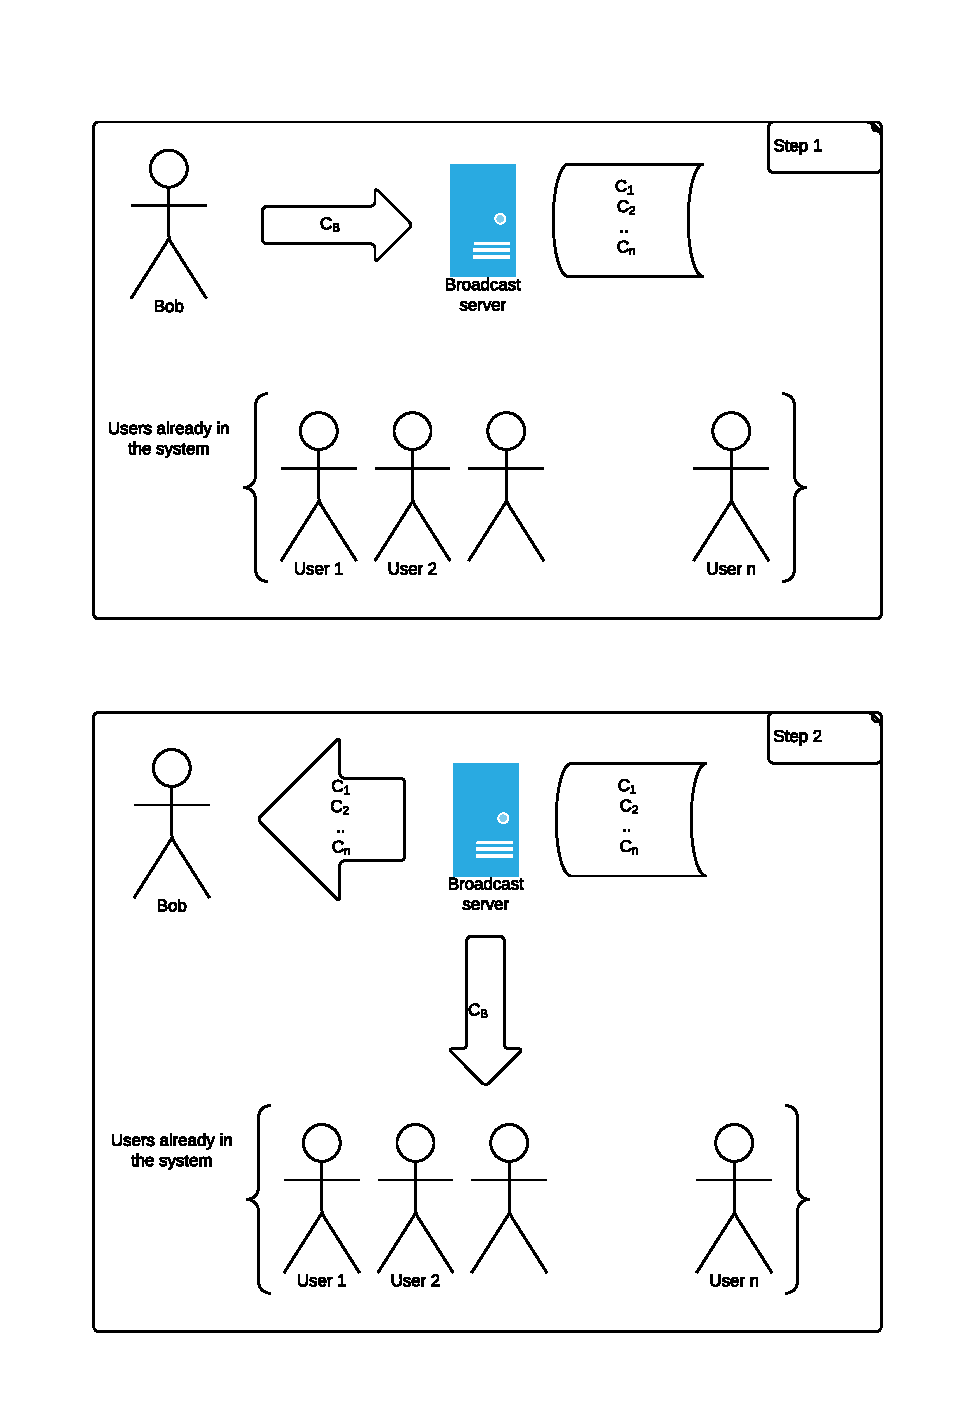
\includegraphics[trim=2cm 1.5cm 2cm 4cm ,scale=1]{chatsystem.pdf}
\caption{Distribution of encapsulations}
\label{fig:encapdistr}
\end{figure}

\begin{figure}
\centering
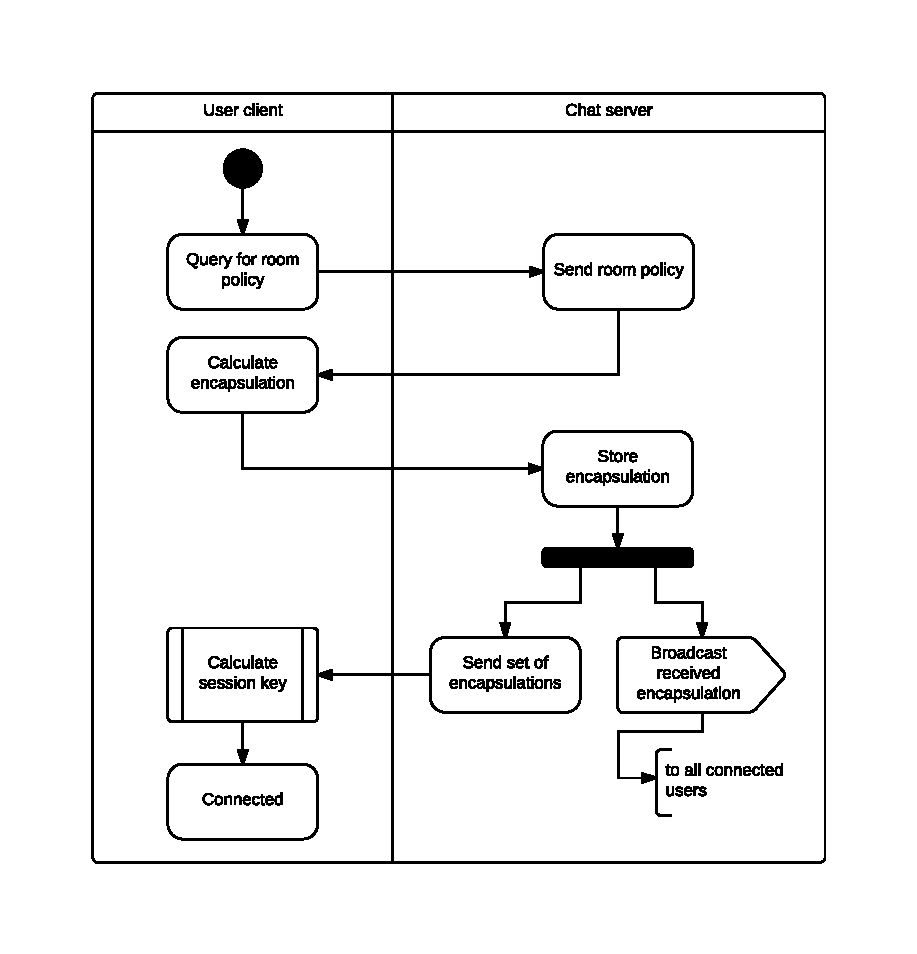
\includegraphics[trim=2cm 2cm 0cm 1cm ,scale=1]{Flow.pdf}
\caption{System flow.}
\label{fig:flow}
\end{figure}
\section{Implementation}
\section{System demonstration}



\chapter{Discussion}\label{cha:discussion}
\renewcommand*{\bibname}{References}
\bibliographystyle{plain}
\bibliography{references/func-key-exchange}
\nocite{*}

%% Uncomment the following if you have any appendix
 \appendix
 \addtocontents{toc}{%
  \protect\vspace{1em}% 
  \protect\noindent \bfseries \appendixtocname\protect\par
  \protect\vspace{-.5em}%
 }
 \renewcommand{\chaptername}{\appendixname}
% include below possible appendices (chapters)
 \chapter{Client.py}\label{clientcode}
\lstinputlisting[language=Python, breaklines=true, tabsize=2, showspaces=false,keywordstyle=\color{green}, basicstyle=\scriptsize]{server.py}

\chapter{Server.py}\label{servercode}
\lstinputlisting[language=Python, breaklines=true, tabsize=2, showspaces=false,keywordstyle=\color{green}, basicstyle=\scriptsize]{client.py}

\end{document} 
